\documentclass{standalone}
\usepackage{tikz}
\usetikzlibrary{patterns, positioning}
\usepackage[sfdefault]{ClearSans} %% option 'sfdefault' activates Clear Sans as the default text font
\usepackage[T1]{fontenc}

\begin{document}
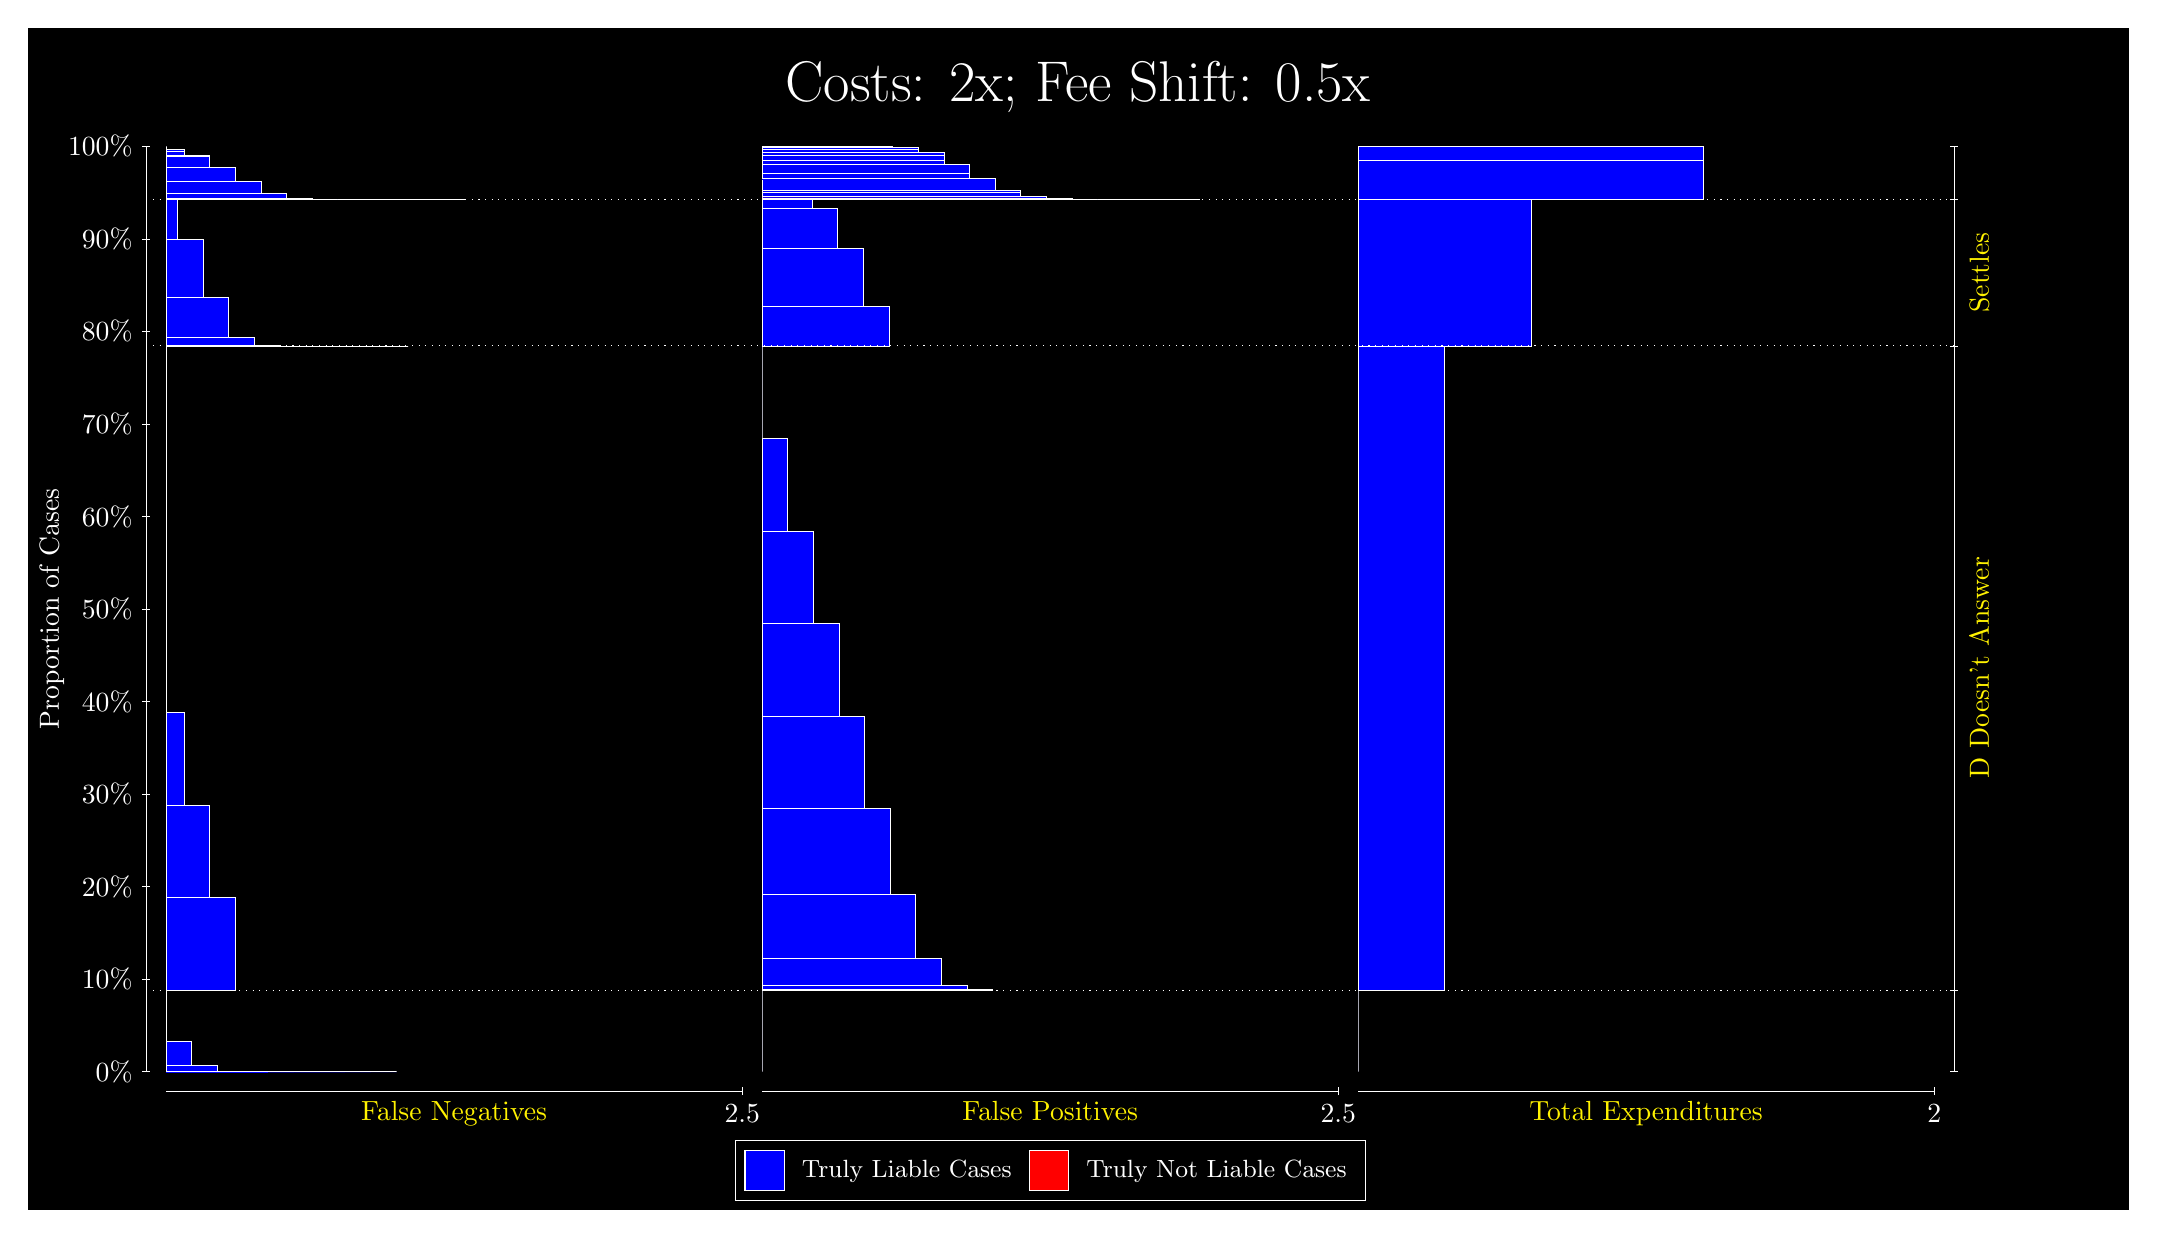
\begin{tikzpicture}
\draw[fill=black] (0,0) rectangle (26.667,15);
\draw[text=white] (0,13.5) rectangle (26.667,15) node[midway] {\huge Costs: 2x; Fee Shift: 0.5x};
\draw[white, very thin] (1.5,1.75) -- (1.5,13.5);
\node[rotate=90, text=white, anchor=center] at (0.3, 7.625) {Proportion of Cases};
\draw[white, very thin] (1.45,1.75) -- (1.55,1.75);
\node[text=white, anchor=east] at (1.45, 1.75) {0\%};
\draw[white, very thin] (1.45,2.925) -- (1.55,2.925);
\node[text=white, anchor=east] at (1.45, 2.925) {10\%};
\draw[white, very thin] (1.45,4.1) -- (1.55,4.1);
\node[text=white, anchor=east] at (1.45, 4.1) {20\%};
\draw[white, very thin] (1.45,5.275) -- (1.55,5.275);
\node[text=white, anchor=east] at (1.45, 5.275) {30\%};
\draw[white, very thin] (1.45,6.45) -- (1.55,6.45);
\node[text=white, anchor=east] at (1.45, 6.45) {40\%};
\draw[white, very thin] (1.45,7.625) -- (1.55,7.625);
\node[text=white, anchor=east] at (1.45, 7.625) {50\%};
\draw[white, very thin] (1.45,8.8) -- (1.55,8.8);
\node[text=white, anchor=east] at (1.45, 8.8) {60\%};
\draw[white, very thin] (1.45,9.975) -- (1.55,9.975);
\node[text=white, anchor=east] at (1.45, 9.975) {70\%};
\draw[white, very thin] (1.45,11.15) -- (1.55,11.15);
\node[text=white, anchor=east] at (1.45, 11.15) {80\%};
\draw[white, very thin] (1.45,12.325) -- (1.55,12.325);
\node[text=white, anchor=east] at (1.45, 12.325) {90\%};
\draw[white, very thin] (1.45,13.5) -- (1.55,13.5);
\node[text=white, anchor=east] at (1.45, 13.5) {100\%};

\draw[white, very thin] (24.457,1.75) -- (24.457,13.5);
\draw[white, very thin] (24.407,1.75) -- (24.507,1.75);
\node[anchor=west] at (24.407, 1.75) {};
\draw[white, very thin] (24.407,2.784) -- (24.507,2.784);
\node[anchor=west] at (24.407, 2.784) {};
\draw[white, very thin] (24.407,10.965) -- (24.507,10.965);
\node[anchor=west] at (24.407, 10.965) {};
\draw[white, very thin] (24.407,12.829) -- (24.507,12.829);
\node[anchor=west] at (24.407, 12.829) {};
\draw[white, very thin] (24.407,13.5) -- (24.507,13.5);
\node[anchor=west] at (24.407, 13.5) {};

\draw[white, very thin, fill=blue] (1.75,1.75) rectangle (4.6775,1.75);
\draw[white, very thin, fill=blue] (1.75,1.75) rectangle (4.3523,1.75);
\draw[white, very thin, fill=blue] (1.75,1.75) rectangle (4.027,1.75);
\draw[white, very thin, fill=blue] (1.75,1.75) rectangle (3.7017,1.75);
\draw[white, very thin, fill=blue] (1.75,1.75) rectangle (3.3764,1.75);
\draw[white, very thin, fill=blue] (1.75,1.75) rectangle (3.0511,1.7503);
\draw[white, very thin, fill=blue] (1.75,1.7503) rectangle (2.7258,1.7573);
\draw[white, very thin, fill=blue] (1.75,1.7573) rectangle (2.4006,1.8289);
\draw[white, very thin, fill=blue] (1.75,1.8289) rectangle (2.0753,2.1333);
\draw[white, very thin, fill=red] (1.75,2.1333) rectangle (1.75,2.1333);
\draw[white, very thin, fill=blue] (1.75,2.1333) rectangle (1.75,2.784);
\draw[white, very thin, fill=blue] (1.75,2.784) rectangle (2.6283,3.959);
\draw[white, very thin, fill=blue] (1.75,3.959) rectangle (2.303,5.134);
\draw[white, very thin, fill=blue] (1.75,5.134) rectangle (1.9777,6.309);
\draw[white, very thin, fill=red] (1.75,6.309) rectangle (1.75,6.309);
\draw[white, very thin, fill=blue] (1.75,6.309) rectangle (1.75,10.965);
\draw[white, very thin, fill=blue] (1.75,10.965) rectangle (4.8239,10.965);
\draw[white, very thin, fill=blue] (1.75,10.965) rectangle (4.4986,10.965);
\draw[white, very thin, fill=blue] (1.75,10.965) rectangle (4.1734,10.965);
\draw[white, very thin, fill=blue] (1.75,10.965) rectangle (3.8481,10.965);
\draw[white, very thin, fill=blue] (1.75,10.965) rectangle (3.5228,10.965);
\draw[white, very thin, fill=blue] (1.75,10.965) rectangle (3.1975,10.97);
\draw[white, very thin, fill=blue] (1.75,10.97) rectangle (2.8722,11.08);
\draw[white, very thin, fill=blue] (1.75,11.08) rectangle (2.5469,11.589);
\draw[white, very thin, fill=blue] (1.75,11.589) rectangle (2.2217,12.319);
\draw[white, very thin, fill=blue] (1.75,12.319) rectangle (1.8964,12.829);
\draw[white, very thin, fill=red] (1.75,12.829) rectangle (1.75,12.829);
\draw[white, very thin, fill=blue] (1.75,12.829) rectangle (5.5558,12.829);
\draw[white, very thin, fill=blue] (1.75,12.829) rectangle (5.2305,12.829);
\draw[white, very thin, fill=blue] (1.75,12.829) rectangle (4.9052,12.829);
\draw[white, very thin, fill=blue] (1.75,12.829) rectangle (4.58,12.829);
\draw[white, very thin, fill=blue] (1.75,12.829) rectangle (4.58,12.829);
\draw[white, very thin, fill=blue] (1.75,12.829) rectangle (4.2547,12.829);
\draw[white, very thin, fill=blue] (1.75,12.829) rectangle (4.2547,12.829);
\draw[white, very thin, fill=blue] (1.75,12.829) rectangle (3.9294,12.829);
\draw[white, very thin, fill=blue] (1.75,12.829) rectangle (3.6041,12.842);
\draw[white, very thin, fill=blue] (1.75,12.842) rectangle (3.2788,12.843);
\draw[white, very thin, fill=blue] (1.75,12.843) rectangle (3.2788,12.908);
\draw[white, very thin, fill=blue] (1.75,12.908) rectangle (2.9535,12.908);
\draw[white, very thin, fill=blue] (1.75,12.908) rectangle (2.9535,12.91);
\draw[white, very thin, fill=blue] (1.75,12.91) rectangle (2.9535,13.054);
\draw[white, very thin, fill=blue] (1.75,13.054) rectangle (2.9535,13.054);
\draw[white, very thin, fill=blue] (1.75,13.054) rectangle (2.6283,13.054);
\draw[white, very thin, fill=blue] (1.75,13.054) rectangle (2.6283,13.239);
\draw[white, very thin, fill=blue] (1.75,13.239) rectangle (2.303,13.239);
\draw[white, very thin, fill=blue] (1.75,13.239) rectangle (2.303,13.24);
\draw[white, very thin, fill=blue] (1.75,13.24) rectangle (2.303,13.372);
\draw[white, very thin, fill=blue] (1.75,13.372) rectangle (2.303,13.388);
\draw[white, very thin, fill=blue] (1.75,13.388) rectangle (1.9777,13.388);
\draw[white, very thin, fill=blue] (1.75,13.388) rectangle (1.9777,13.438);
\draw[white, very thin, fill=blue] (1.75,13.438) rectangle (1.9777,13.466);
\draw[white, very thin, fill=red] (1.75,13.466) rectangle (1.75,13.466);
\draw[white, very thin, fill=blue] (1.75,13.466) rectangle (1.75,13.5);
\draw[white, very thin, fill=red] (9.3189,1.75) rectangle (9.3189,1.75);
\draw[white, very thin, fill=blue] (9.3189,1.75) rectangle (9.3189,2.784);
\draw[white, very thin, fill=red] (9.3189,2.784) rectangle (12.246,2.784);
\draw[white, very thin, fill=blue] (9.3189,2.784) rectangle (12.246,2.7887);
\draw[white, very thin, fill=blue] (9.3189,2.7887) rectangle (11.921,2.851);
\draw[white, very thin, fill=blue] (9.3189,2.851) rectangle (11.596,3.1936);
\draw[white, very thin, fill=blue] (9.3189,3.1936) rectangle (11.271,4.0014);
\draw[white, very thin, fill=blue] (9.3189,4.0014) rectangle (10.945,5.0976);
\draw[white, very thin, fill=blue] (9.3189,5.0976) rectangle (10.62,6.2653);
\draw[white, very thin, fill=blue] (9.3189,6.2653) rectangle (10.295,7.4401);
\draw[white, very thin, fill=blue] (9.3189,7.4401) rectangle (9.9694,8.6151);
\draw[white, very thin, fill=blue] (9.3189,8.6151) rectangle (9.6442,9.7901);
\draw[white, very thin, fill=blue] (9.3189,9.7901) rectangle (9.3189,10.965);
\draw[white, very thin, fill=red] (9.3189,10.965) rectangle (10.929,10.965);
\draw[white, very thin, fill=blue] (9.3189,10.965) rectangle (10.929,11.474);
\draw[white, very thin, fill=blue] (9.3189,11.474) rectangle (10.604,12.204);
\draw[white, very thin, fill=blue] (9.3189,12.204) rectangle (10.278,12.714);
\draw[white, very thin, fill=blue] (9.3189,12.714) rectangle (9.9532,12.823);
\draw[white, very thin, fill=blue] (9.3189,12.823) rectangle (9.6279,12.829);
\draw[white, very thin, fill=blue] (9.3189,12.829) rectangle (9.3189,12.829);
\draw[white, very thin, fill=red] (9.3189,12.829) rectangle (14.881,12.829);
\draw[white, very thin, fill=blue] (9.3189,12.829) rectangle (14.881,12.829);
\draw[white, very thin, fill=red] (9.3189,12.829) rectangle (14.556,12.829);
\draw[white, very thin, fill=blue] (9.3189,12.829) rectangle (14.556,12.829);
\draw[white, very thin, fill=red] (9.3189,12.829) rectangle (14.231,12.829);
\draw[white, very thin, fill=blue] (9.3189,12.829) rectangle (14.231,12.829);
\draw[white, very thin, fill=blue] (9.3189,12.829) rectangle (13.905,12.829);
\draw[white, very thin, fill=red] (9.3189,12.829) rectangle (13.905,12.829);
\draw[white, very thin, fill=blue] (9.3189,12.829) rectangle (13.905,12.829);
\draw[white, very thin, fill=red] (9.3189,12.829) rectangle (13.58,12.829);
\draw[white, very thin, fill=blue] (9.3189,12.829) rectangle (13.58,12.829);
\draw[white, very thin, fill=blue] (9.3189,12.829) rectangle (13.58,12.829);
\draw[white, very thin, fill=red] (9.3189,12.829) rectangle (13.255,12.829);
\draw[white, very thin, fill=blue] (9.3189,12.829) rectangle (13.255,12.833);
\draw[white, very thin, fill=blue] (9.3189,12.833) rectangle (13.255,12.835);
\draw[white, very thin, fill=blue] (9.3189,12.835) rectangle (12.93,12.846);
\draw[white, very thin, fill=red] (9.3189,12.846) rectangle (12.93,12.846);
\draw[white, very thin, fill=blue] (9.3189,12.846) rectangle (12.93,12.862);
\draw[white, very thin, fill=red] (9.3189,12.862) rectangle (12.604,12.862);
\draw[white, very thin, fill=blue] (9.3189,12.862) rectangle (12.604,12.922);
\draw[white, very thin, fill=blue] (9.3189,12.922) rectangle (12.604,12.941);
\draw[white, very thin, fill=red] (9.3189,12.941) rectangle (12.279,12.941);
\draw[white, very thin, fill=blue] (9.3189,12.941) rectangle (12.279,13.088);
\draw[white, very thin, fill=blue] (9.3189,13.088) rectangle (12.279,13.09);
\draw[white, very thin, fill=blue] (9.3189,13.09) rectangle (11.954,13.159);
\draw[white, very thin, fill=red] (9.3189,13.159) rectangle (11.954,13.159);
\draw[white, very thin, fill=blue] (9.3189,13.159) rectangle (11.954,13.275);
\draw[white, very thin, fill=blue] (9.3189,13.275) rectangle (11.954,13.275);
\draw[white, very thin, fill=blue] (9.3189,13.275) rectangle (11.628,13.328);
\draw[white, very thin, fill=blue] (9.3189,13.328) rectangle (11.628,13.384);
\draw[white, very thin, fill=blue] (9.3189,13.384) rectangle (11.628,13.42);
\draw[white, very thin, fill=blue] (9.3189,13.42) rectangle (11.628,13.42);
\draw[white, very thin, fill=blue] (9.3189,13.42) rectangle (11.303,13.457);
\draw[white, very thin, fill=blue] (9.3189,13.457) rectangle (11.303,13.486);
\draw[white, very thin, fill=blue] (9.3189,13.486) rectangle (11.303,13.487);
\draw[white, very thin, fill=blue] (9.3189,13.487) rectangle (10.978,13.499);
\draw[white, very thin, fill=blue] (9.3189,13.499) rectangle (10.978,13.499);
\draw[white, very thin, fill=blue] (9.3189,13.499) rectangle (10.978,13.499);
\draw[white, very thin, fill=blue] (9.3189,13.499) rectangle (10.653,13.499);
\draw[white, very thin, fill=blue] (9.3189,13.499) rectangle (10.653,13.5);
\draw[white, very thin, fill=blue] (9.3189,13.5) rectangle (10.653,13.5);
\draw[white, very thin, fill=blue] (9.3189,13.5) rectangle (10.327,13.5);
\draw[white, very thin, fill=blue] (9.3189,13.5) rectangle (10.327,13.5);
\draw[white, very thin, fill=blue] (9.3189,13.5) rectangle (10.002,13.5);
\draw[white, very thin, fill=blue] (9.3189,13.5) rectangle (10.002,13.5);
\draw[white, very thin, fill=blue] (9.3189,13.5) rectangle (10.002,13.5);
\draw[white, very thin, fill=blue] (9.3189,13.5) rectangle (9.6767,13.5);
\draw[white, very thin, fill=blue] (9.3189,13.5) rectangle (9.6767,13.5);
\draw[white, very thin, fill=blue] (9.3189,13.5) rectangle (9.3514,13.5);
\draw[white, very thin, fill=blue] (9.3189,13.5) rectangle (9.3189,13.5);
\draw[white, very thin, fill=red] (16.888,1.75) rectangle (16.888,1.75);
\draw[white, very thin, fill=blue] (16.888,1.75) rectangle (16.888,2.784);
\draw[white, very thin, fill=red] (16.888,2.784) rectangle (17.986,2.784);
\draw[white, very thin, fill=blue] (16.888,2.784) rectangle (17.986,10.965);
\draw[white, very thin, fill=red] (16.888,10.965) rectangle (19.083,10.965);
\draw[white, very thin, fill=blue] (16.888,10.965) rectangle (19.083,12.829);
\draw[white, very thin, fill=red] (16.888,12.829) rectangle (21.279,12.829);
\draw[white, very thin, fill=blue] (16.888,12.829) rectangle (21.279,13.323);
\draw[white, very thin, fill=red] (16.888,13.323) rectangle (21.279,13.323);
\draw[white, very thin, fill=blue] (16.888,13.323) rectangle (21.279,13.5);
\draw[white, dotted] (1.5,2.784) -- (24.457,2.784);
\draw[white, dotted] (1.5,10.965) -- (24.457,10.965);
\draw[white, dotted] (1.5,12.829) -- (24.457,12.829);
\draw[white, very thin] (1.75,1.5) -- (9.0689,1.5);
\node[text=yellow, anchor=north] at (5.4094, 1.5) {False Negatives};
\draw[white, very thin] (9.0689,1.45) -- (9.0689,1.55);
\node[text=white, anchor=north] at (9.0689, 1.45) {2.5};

\draw[white, very thin] (9.3189,1.5) -- (16.638,1.5);
\node[text=yellow, anchor=north] at (12.978, 1.5) {False Positives};
\draw[white, very thin] (16.638,1.45) -- (16.638,1.55);
\node[text=white, anchor=north] at (16.638, 1.45) {2.5};

\draw[white, very thin] (16.888,1.5) -- (24.207,1.5);
\node[text=yellow, anchor=north] at (20.547, 1.5) {Total Expenditures};
\draw[white, very thin] (24.207,1.45) -- (24.207,1.55);
\node[text=white, anchor=north] at (24.207, 1.45) {2};


\node[text=yellow, centered, rotate=90] at (24.777, 6.8745) {D Doesn't Answer};
\node[text=yellow, centered, rotate=90] at (24.777, 11.897) {Settles};


\draw (12.978300999999998,1.5) node[draw=none] (baseCoordinate) {};
\begin{scope}[align=center]
        \matrix[scale=0.5, draw=white, below=0.5cm of baseCoordinate, nodes={draw}, column sep=0.1cm]{
            \node[rectangle, draw, minimum width=0.5cm, minimum height=0.5cm, fill=blue] {}; &
            \node[draw=none, font=\small, text=white] (B) {Truly Liable Cases}; &
            \node[rectangle, draw, minimum width=0.5cm, minimum height=0.5cm, fill=red] {}; &
            \node[draw=none, font=\small, text=white] (B) {Truly Not Liable Cases}; \\
            };
\end{scope}

\end{tikzpicture}
\end{document}